\section{Implementation}
\label{sec:implementation}

We have implemented the NDN-IoT framework and a prototype of the Flow entertainment experience to verify the design introduced in the previous section.
The implementation follows a modular structure and differentiates between the framework-level services that we believe are common to many home IoT systems and the functionality that supports Flow-specific application logic.
This section describes details in both the framework, and components of the application.

\subsection{NDN-IoT framework}

The NDN-IoT framework includes an implementation of the authentication server, as well as a set of client libraries using JavaScript, Python, C\# and C++.
The NDN-IoT client libraries are built on top of the NDN Common Client Libraries~\cite{ccl}, and aims to provide abstractions to faciliate application development in a home environment. 
The client libraries in four languages are organized into three major functional blocks:
\begin{enumerate}
\item \textit{Bootstrap}
\item \textit{Discovery}
\item \textit{Application-level pub/sub}
\end{enumerate}

The AS is based on the team's previous work on NDN-pi (citation: ndn-pi TR). The framework provides a server implementation in Python, since we run the AS on Rasperry Pi. Authentication clients are available in both Python and JavaScript, so that we can support application components running on Ubuntu, OSX, Raspbian, and browser platforms.

Compared with NDN-pi, the AS implementation made the following updates (insert details), and provided a similar functioning port in JavaScript.

\subsection{Flow application components}

% Subsystems
In our prototype, each of the Flow application components is implemented as the following:
\begin{enumerate}
\item \textit{Indoor positioning}: We use OpenPTrack,\footnote{\url{http://openptrack.org/about/}} a multi-camera person tracking system.
The NDN producer for OpenPTrack\footnote{\url{https://github.com/OpenPTrack/ndn-opt/}} (written in C++)  publishes the position of each person at a 30Hz rate, along with lower rate metadata about active tracks. 
% Interest pipelining and an application-level Pending Interest Table are used for real-time delivery of position data.
% Dealing with constrained devices: better in design or implementation? deserve its own paragraph and figure?
\item \textit{Wearable sensing}: We use an RFduino 22301 with gyroscope MPU6050 attached to provide virtual camera control. 
The RFduino cannot perform asynchronous signing operations quickly enough, so we introduced a Raspberry Pi controller as a gateway for bridging RFduino to the NDN home network.
The data exchanged between RFduino and Raspberry Pi is signed with a shared secret key negotiated after Bluetooth pairing.
The Raspberry Pi generates a public/private key pair on behalf of the RFduino to be associated with the RFduino's device identity.
The RFduino runs a minimum NDN producer, implemented with the ndn-cpp-lite library\footnote{\url{https://github.com/named-data/ndn-cpp/}}, which generates data at roughly 2Hz rate.
When new data is generated, the RFduino pushes the data (signed by the pre-negotiated shared secret) to the Raspberry Pi controller over the Bluetooth LE channel.
The controller receives the data, repackages the data and signs the data using RFduino's private key, and then publishes the data on the home network.
The RFduino data publishing process is shown in Fig.~\ref{fig:contrained-devices-bootstrap}.
% More reasons needed for matching between IDs?
\item \textit{Mobile phone interface}: We employ an Android phone that loads a control webpage (written in JavaScript) in a mobile browser to interact with the virtual environment. 
The phone sends out two types of command Interests: the first one matches an OpenPTrack track ID with that of the mobile, and the second one drops an image onto the virtual environment where the user's avatar is standing. ID matching is introduced so that the visualization knows the location of the user's avatar (identified by a track ID) when an image drop command Interest is issued by the same user (identified by the mobile's ID).
\item \textit{Visualization}: We use the Unity3D\footnote{\url{https://unity3d.com}} game engine for visualization.
The game engine runs C\# NDN data consumers that receive person tracking and virtual camera control data, and a producer that receives image dropping command Interests from the mobile web interface.
\end{enumerate}

\begin{figure}[!t]
\centering
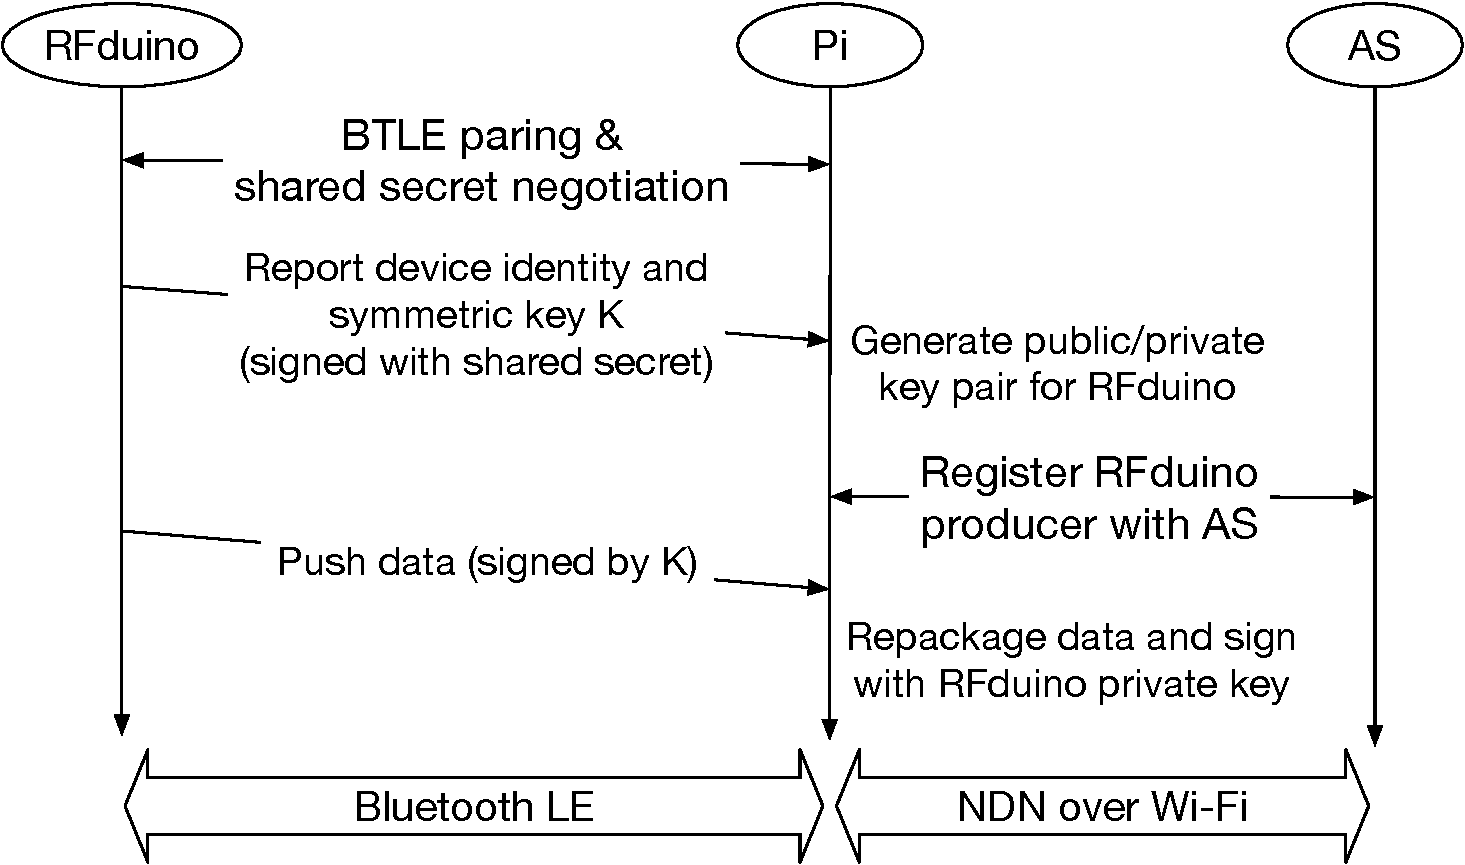
\includegraphics[width=0.95\columnwidth]{constrained-device-authorization.pdf}
\caption{RFduino data publishing with assistance of Raspberry Pi controller}
\label{fig:contrained-devices-bootstrap}
\end{figure}

The implementation for both NDN-IoT framework and Flow application are available online.\footnote{\url{https://github.com/remap/ndn-flow}} We installed two instances of the Flow application testbed at UCLA and Huawei. Fig.~\ref{fig:message-flow-in-flow-installation} shows a diagram of the system and its message flows after all devices are bootstrapped with an AS, which in our installation is another Raspberry Pi.

\begin{figure*}[!t]
\centering
\includegraphics[width=0.95\textwidth]{flow-components-ndn-names-diagram-zs.pdf}
\caption{Application components and message flows in Flow}
\label{fig:message-flow-in-flow-installation}
\end{figure*}
